\documentclass[20 pts]{article}
%\usepackage{xeCJK}
\usepackage{amsfonts}
\usepackage{amssymb}
\usepackage{csvsimple}
\usepackage{caption}
\usepackage{longtable}
\usepackage{amsmath}
\usepackage{bm}
\usepackage{graphicx}
%\setCJKmainfont{SimSun}
\title{Deterministic Interleaver Design for Turbo Codes} 
\author{Kwame Ackah Bohulu, 1631133}
\date{22-06-2017}


\begin{document}
\maketitle
\newpage
\section{Abstract}
input weight 2m error events with the distance between the bit '1' seperated by a 
multiple of
the componet codes cycle length ($a-\tau$ seperated input weight 2m error events) 
tend to produce low-weight turbo codewords if present
in both component codes. In this research paper, we introduce a 
method for designing deterministic
interleavers for turbo codes in such a way that $a-\tau$ seperated input weight 2m 
error events in 
the first component encoder are not mapped unto the second component encoder. 
Using
this method, we find good interleavers for specified frame lengths and component 
codes. The performance of the designed interleavers is tested against the Quadratic 
Permutation Polynomial (QPP) Interleaver and is shown to be better especially for long
frame sizes.

\section{Introduction}
Turbo Codes are amongst the class of capacity approaching FEC codes that were 
discovered in 1993 by Claude Bearoux. They are constructed by the parallel 
concatenation of 2 Recursive Systematic Convolutional (RSC) Encoders via an 
interleavers. Diagram for 


Decoding of Turbo codes is done using the Turbo Decoder. It is made up 2 Soft 
Input Soft 
Output (SISO) Decoders.
The interleaver plays a very important role in Turbo codes as it reduces the number of
 low-weight codewords(multiplicity) of the Turbo code [4]. However, the existence of 
 the low-weight codewords causes the turbo codes to have a high error floor in the 
 high SNR region. A lot of research has been done concerning interleavers for 
 turbo codes and they are generally put into 2 groups, Random and 
 Deterministic interleavers.
\paragraph{}
Turbo codes implemented using Random interleavers have been shown to have good
 performance, especially for large frame sizes [3]. The disadvantage of using 
 Random interleavers stems from required use of interleaver tables in both the 
 encoder and decoder, which is undesirable in many applications. 
 Deterministic interleaver
  on the other hand require no such interleaver tables and the logic behind interleaving
   and deinterleaving can be executed by means of algorithms. Due to this advantage, 
   a lot of Turbo codes employ Deterministic interleavers in their construction. Most 
   noticable amongst these is the Quadratic Permutation Polynomial (PP2) 
   interleaver [3]
    which is used in LTE applications.
\paragraph{}
Despite this advantage, Deterministic interleavers that outperform Random interleavers,
 especially for large frame sizes have yet to be discovered. The aim of this research is
  to design an interleaver that has a performance that is at least as good as that of 
  random 
  interleavers for large frame sizes. 

\subsection{Turbo Encoding and Decoding}
The Turbo encoder is shown in figure (\ref{TC}).

\begin{center}
\begin{figure}[h!]
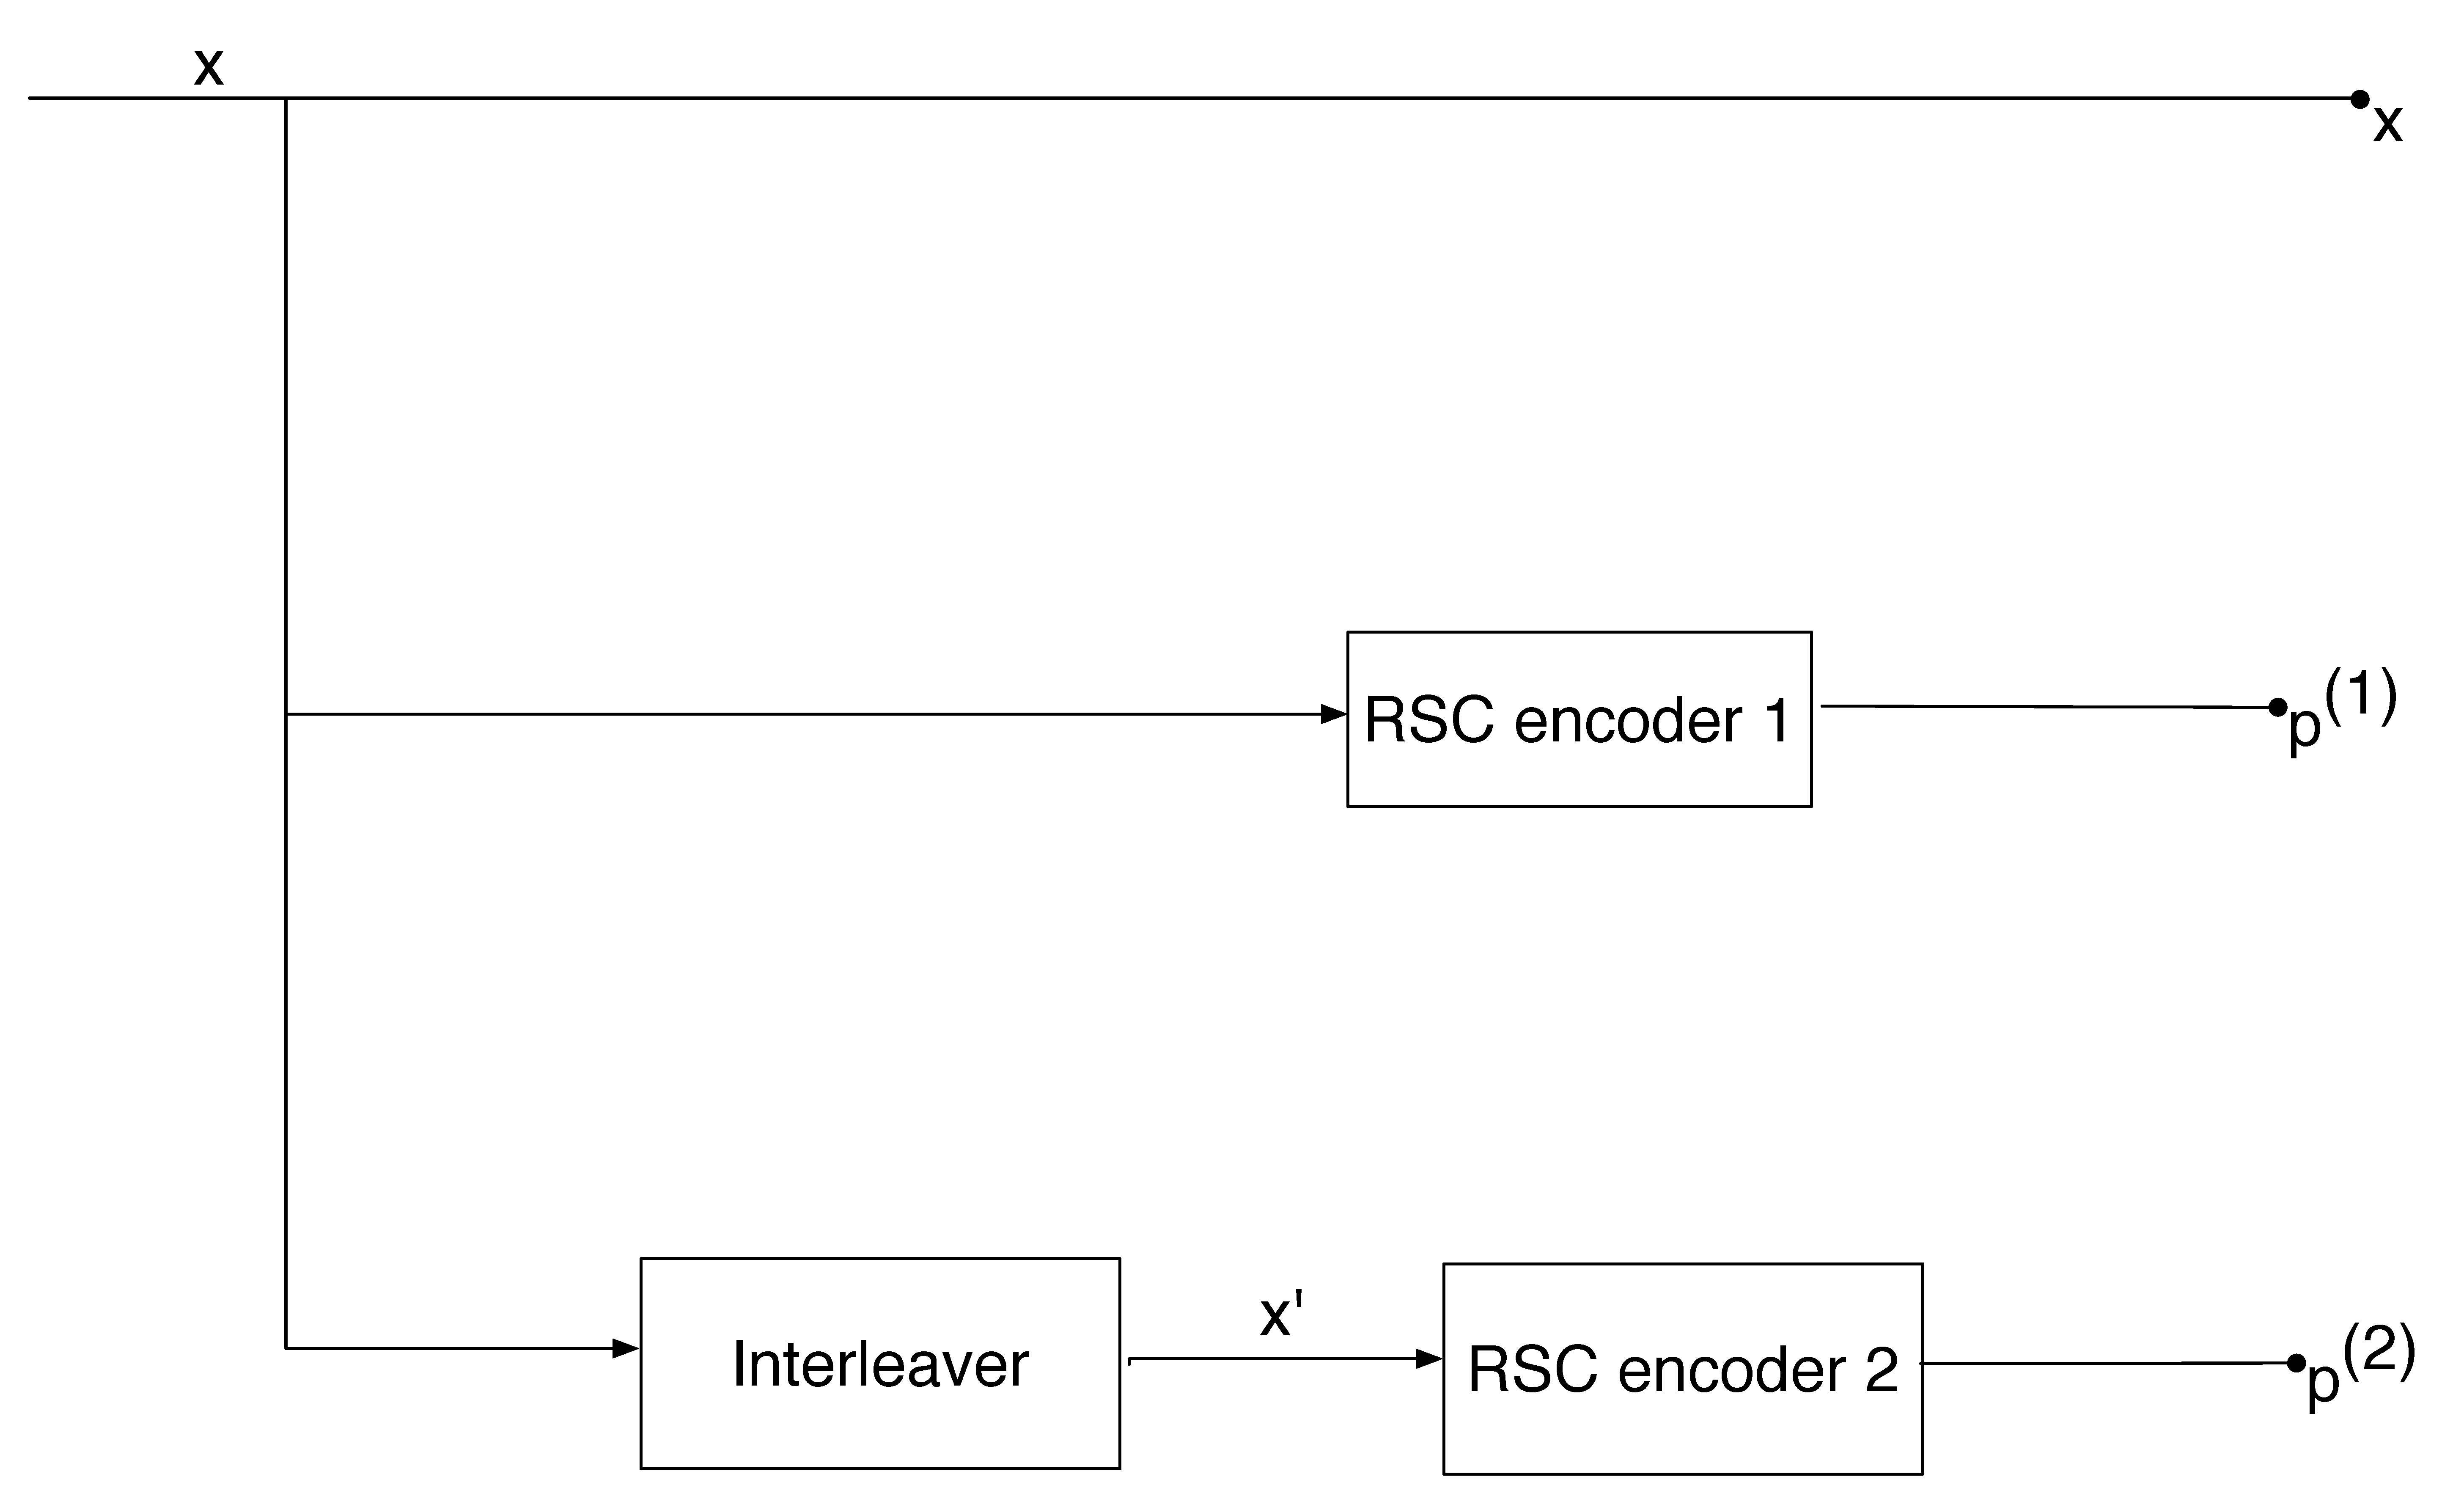
\includegraphics[width=8cm]{TurboEncoder.pdf}
\caption{Turbo Encoder}
\label{TC}
\end{figure}
\end{center}
\paragraph{}The component encoders (CEs) used are identical (N+$m_{RSC}$, N) 
RSC encoders with the 
generator matrix given in octal form $\frac{d}{e}$ where e is the feedback vector 
,d is
the feedforward vector and $m_{RSC}$ is the memory order of the RSC encoder. 
In our
encoding scheme, we wish to return the CEs to the all-zero state.This is acheived by
using $m_{RSC}$ non-zero tail bits. The turbo encoding process is as follows.
The binary input information (systematic) 
sequence $\mathbf{u}=\{u_1, u_2,...,u_{N-1}, u_N \}$ of
 length N is fed into each CE. The upper CE receives the
  input as is and produces the upper parity bit sequence 
  $\mathbf{v}=\{v_1, v_2,...,v_{N-1}, v_N,...,v_{N+m_{RSC}} \}$
  of length N+$m_{RSC}$ . The input to
  the lower CE is an interleaved version of the input information sequence 
  $\mathbf{u}'=\{u'_1, u'_2,...,u'_{N-1}, u'_N \}$. This is used to generate the 
  lower parity bit sequence 
  $\mathbf{v}'=\{v'_1, v'_2,...,v'_{N-1}, v'_N,...,v'_{N+m_{RSC}} \}$ also
  of length N+$m_{RSC}$. The output rate of the turbo code using this encoding
  scheme is $\frac{N}{3N+2m_{RSC}}$. The systematic, upper and lower parity bits 
  are multiplexed and modulated using BPSK and transmitted over the AWGN channel.

\paragraph{}
Decoding of turbo codes is done using the turbo decoding algorithm. This algorithm
is based on the iterative use of the BCJR algorithm or variations of it. 
In this research we
use the Max-Log-APP algorithm as described in [].

Assuming BPSK modulation and transmission over the AWGN channel
the a posteriori LLR values are calculated using the equation below.
\begin{equation}
L(u_i)=L_cy^s_i + L_a (u_i) + L_e(u_i)
\label{LLR}
\end{equation}
The meaning and definitions of all variables related to (\ref{LLR}) are summarized in
Table \ref{LLR}.

\begin{table}[h!]
\begin{center}
 \begin{tabular}{|| c | c | c | c ||} 
 
 \hline
 variable & definition & formula & initial values  \\ [0.5ex] 
 \hline\hline
 $L_cy^s_i$ & 0 0 $\rightarrow$ 1 0 & 1 0 $\rightarrow$ 1 1 & 1 1 $\rightarrow$ 0 1  \\ 
 \hline
 $L_a (u_i)$  & 0 0 $\rightarrow$ 0 0 & 0 0 $\rightarrow$ 1 0 & 1 0 $\rightarrow$ 0 1  \\ 
 \hline
  $L_e(u_i)$& 0 0 $\rightarrow$ 1 0 & 1 0 $\rightarrow$ 0 1 & 0 1 $\rightarrow$ 1 0  \\ [1ex] 
 \hline
 
\end{tabular}
\label{T1}
\end{center}
\label{T1}
\caption{$d_k = 0$}
\end{table}

The Turbo decoder is shown in Figure \ref{TD}.
\begin{figure}[h!]
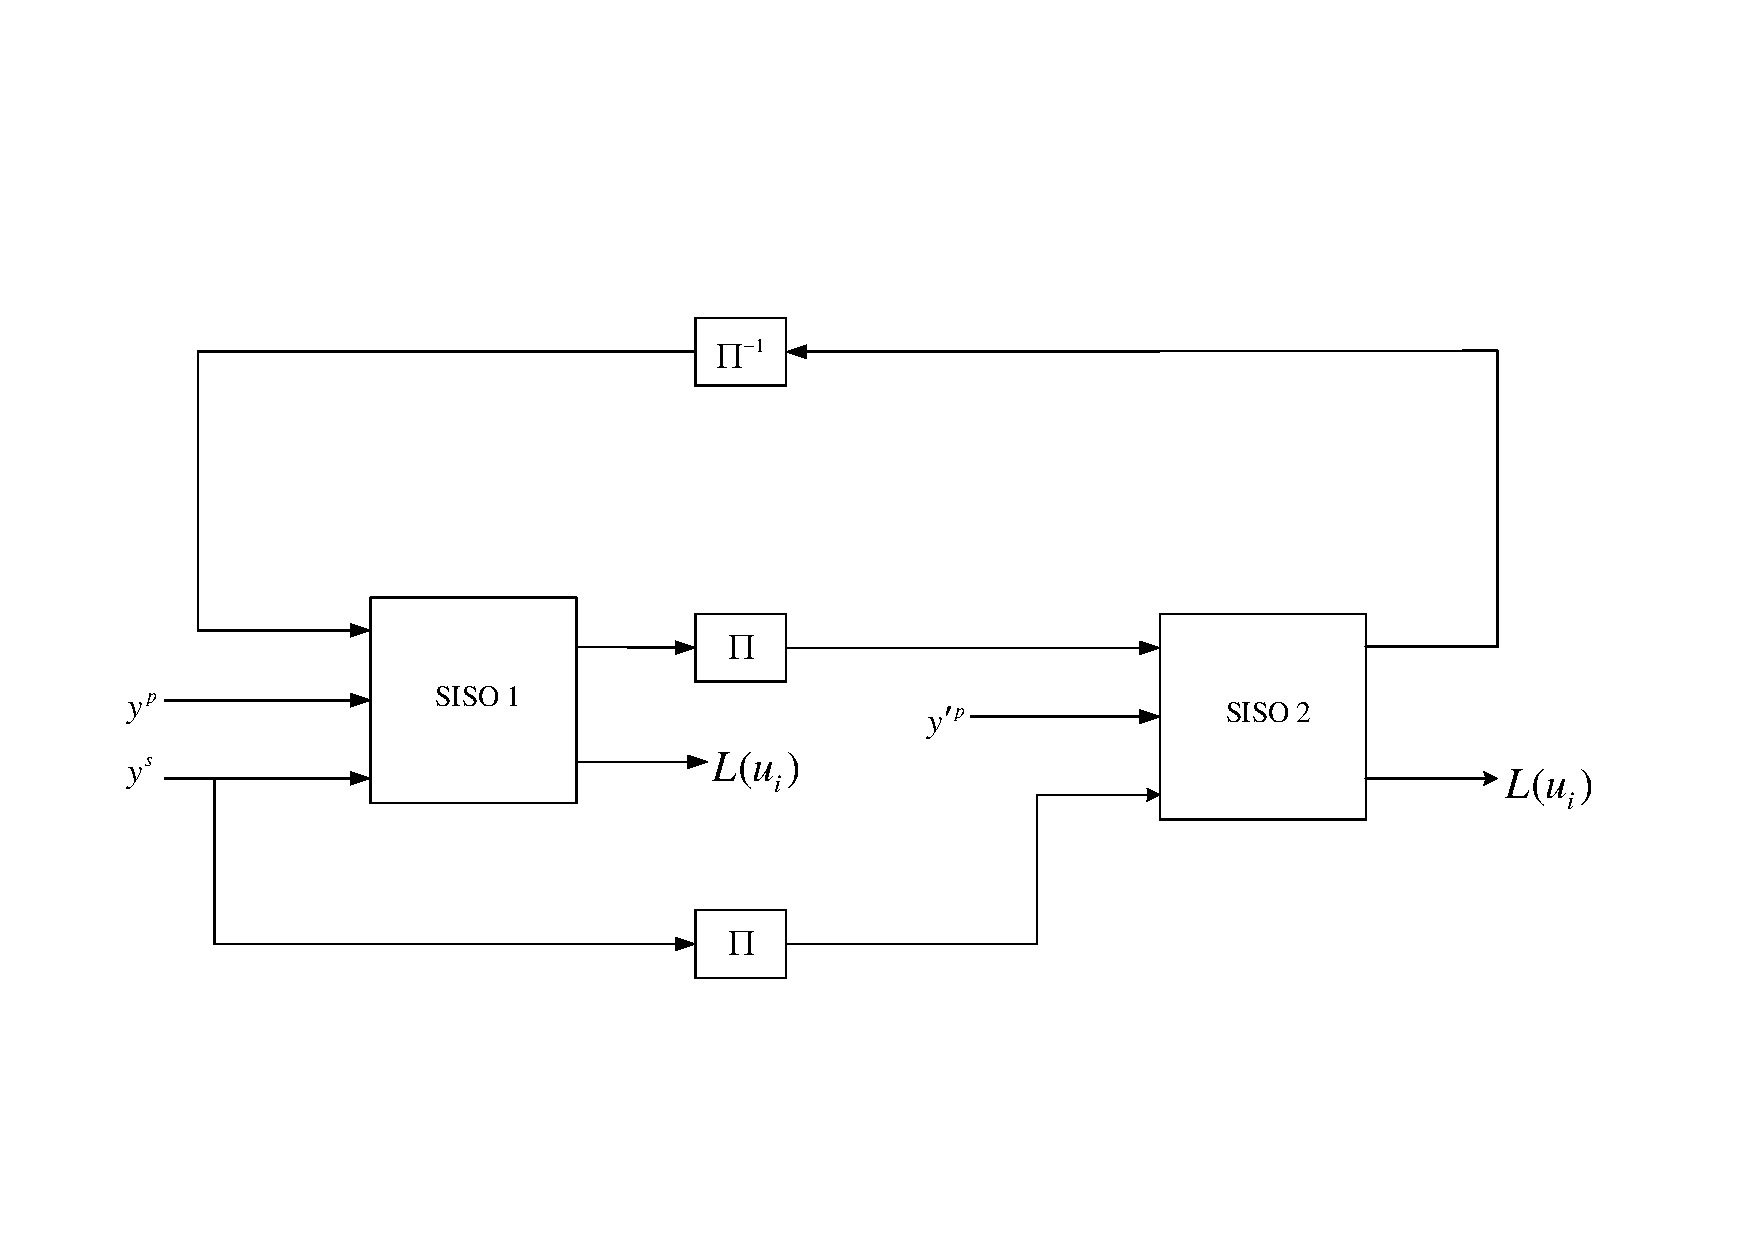
\includegraphics[width=10cm]{D1.pdf}
\caption{Turbo Decoder}
\label{TD}
\label{図2}
\end{figure}
it utilises 2 Soft Input Soft Output (SISO) decoders(one for each encoder) 
connected in such
a way that the $L_e(\mathbf{u})$ from one encoder is fed into the other as
 $L_a(\mathbf{u})$.
 \paragraph{}
 The turbo code transmitted over the AWGN channel is received as
  $\mathbf{y}=\{\mathbf{y_u},\mathbf{y_v},\mathbf{y_{v'}} \}$ of length 
  $3N +2m_{RSC}$, where $\mathbf{y_u},\mathbf{y_v},\mathbf{y_{v'}}$
    correspond to the systematic, upper and lower parity bits respectively.
    $$\mathbf{y_u}=\{y_{u_1}, y_{u_2},...,y_{u_{N-1}}, y_{u_N} ,...,y_{u_{N+m_{RSC}}}\}$$ 
     $$\mathbf{y_v}=\{y_{v_1}, y_{v_2},...,y_{v_{N-1}}, y_{v_N} ,...,y_{v_{N+m_{RSC}}}\}$$
      $$\mathbf{y_{v'}}=\{y_{{v'}_1}, y_{{v'}_2},...,y_{{v'}_{N-1}}, y_{{v'}_N},...,y_{{v'}_{N+m_{RSC}}} \}$$ 
    
  The decoding process is as follows.
  

The input to the SISO1 is $\mathbf{y_u},\mathbf{y_v}$ and $\mathbf{L_a}$. 
For the first iteration, it is assumed 
that the input information bits have equal probability and $\mathbf{L_a}$ is an 
all-zero vector.
These are used to calculate $\boldsymbol{\gamma },\boldsymbol{\alpha} , 
\boldsymbol{\beta} $
 and finally
$\mathbf{L}$ using (\ref{LLR}) and $\mathbf{L_e^{(1)}}$ is obtained by subtracting
 $L_cy_i^s$  from each element in $\mathbf{L}$.
$\mathbf{L_e^{(1)}}$ is then
 interleaved and fed into SISO2 as the value for
 $\mathbf{L_a}$ along with an interleaved version of $\mathbf{y_u}$ and 
 $ \mathbf{y_{v'}}$ which correspond to
 the interleaved systematic bits and the lower parity bits. These are used to calculate 
 $\boldsymbol{\gamma },\boldsymbol{\alpha} , 
\boldsymbol{\beta},\mathbf{L}$
 and finally the extrinsic LLR values 
of the second component decoder, $\mathbf{L_e^{(2)}}$.
$\mathbf{L_e^{(2)}}$is deinterleaved、and fedback into the first component encoder
 as the new $\mathbf{L_a}$ value for SISO1.
\paragraph{}
The process is either repeated for a predetermined number of times, or untill a certain 
condition is met. At the final iteration $\mathbf{L}$ (from the second component
 decoder) is deinterleaved and used to estimate the values of $\mathbf{u}$.

\section{a-$\tau$ seperated weight 2m error events}
The component encoder of choice for Turbo codes is the Recursive Systematic 
Convolutional (RSC) encoder. The system diagram is shown in the figure below. The
generator matrix is of the form 
$$[1\,  \, \frac{F(D)}{G(D)}]$$ where F(D) represents the 
feed-forward portion of the encoder and G(D) the feed-back portion of the encoder.''1''
represents the systematic input which is also present in the output of the code. In this 
paper we will describe the RSC encoders generator matrix by the feed-foward and 
feed-back portion and in the  octal form.

Each RSC encoder has a cyclic length, which is defined as the parity output of the
 encoder when the input is [1,0,0,...]. For the 5/7 RSC encoder, the output is
 [1,1,1,0,1,1,0,1,1,0...]. We observe an output cycle of [1,1,0] which gives a cycle 
 length($\tau$) of 3. Now, if a weight-2 input sequence with the ''1'' bits separated 
 by a$\tau$ -1 ''0'' bits (a-$\tau$ separated input weight -2 error event, a={1,2,3}) ,
 a low-weight codeword is output. An example is shown in the figure below. In the
 case where an error event in CE1 is mapped unto CE2 by the interleaver ,a 
 low-weight turbo codeword is produced. Since the performance of turbo codes at
 high SNR is dependent on the lowest weight codeword, we wish to avoid such
 cases. To acheive this, it is necessary to design an interleaver that prevents the 
 mapping of a-$\tau$ separated input weight -2 error event in CE1 unto CE2. For
 simplicity sake, we shall refer to a-$\tau$ separated input weight -2 error event as
 a-$\tau$ error event from here onwards.
 
\section{ BER Performance Bounds for Turbo Codes via Union Bound}
Assuming BPSK modulation and the transmission of the all-zero sequence
over the AWGN channel, the union bound BER performance of a turbo code is 
 bounded by[Proakis]
 
 $$P_b \leq \frac{1}{N} \sum_{m=1}^{2^N-1} w^{(s)}_{m} Q\Bigg(\sqrt{2R_cw^{(c)}_{m}\frac{E_b}{N_o}}\Bigg)$$
where $w^{(s)}_m$,$w^{(c)}_m$,$R_c$ , $\frac{E_b}{N_o}$are the weight of the mth information
 sequence, weight of the codeword generated from the mth information sequence, the overall 
 coding rate and the bit energy to noise ratio of the channel respectively. N is the length of the 
 information sequence.
 
 The above equation may be written to group infromation sequences of the same 
 weight. This gives rise to the equation below
 
 \begin{equation}
P_b \leq \frac{1}{N} \sum_{m=1}^{N} \sum_{l=1}^{\binom{N}{m}}mQ\Bigg(\sqrt{2R_cw^{(c)}_{ml}\frac{E_b}{N_o}}\Bigg)
 \end{equation}
 
where $\binom{N}{m}$,and $w^{(c)}_{ml}$ are the number of information 
sequences of weight m and the weight of the codeword generated by the lth information
sequence of weight m.
\section{Methodology}
Turbo codes have error floor in the high SNR region. This has been attributed to the 
prescence of low-weight codewords. The error floor of the Turbo codes can be raised
 by increasing the interleaver size whiles maintaining the effective free distance. 
 Alternatively increasing the effective free distance of the Turbo while maintaining the 
 multiplicity serves a similar purpose [2]. The effective free distance of a code is the
  minimum distance associated with an input of weight 2. 
\paragraph{}
In RSC encoders, weight 2 inputs of the form 
$(1+D^{t\tau})(D^u) ,0\leq u\leq N-\tau, t=\{1,2,3,...\}$
 tend
 to produce low-weight codeword [1]. $\tau$ is the cycle length of the RSC encoder. 
 We shall call such low-weight producing weight 2 inputs $a-\tau$-seperated input 
 weight 2 errors. If the $a-\tau$-seperated input weight 2 errors are input into the 
 Turbo codes component encoders a low-weight codeword will be produced. 

To increase effective free distance of the turbo code, we design an interleaver in such 
a way that the input to the second is of the form 
\begin{equation}
(1+D^{c\tau})(D^u) ,0\leq u\leq N-\tau
\label{one}
\end{equation}
where $c$ is a large number.

\subsection{Linear interleaver design}
The mapping function for the linear interleaver is given by
\begin{equation}
\Pi_{\mathbf{L}_n}(i) \equiv bi  \mod N, \ 0 \leq i \leq N
\label{two}
\end{equation}
where $b$ is a positive integer that is co-prime to $N$. 
The simplest $a-\tau$-seperated input weight 2 error (t=1) is shown in the figure 
below.

\begin{center}
\begin{figure}[h!]
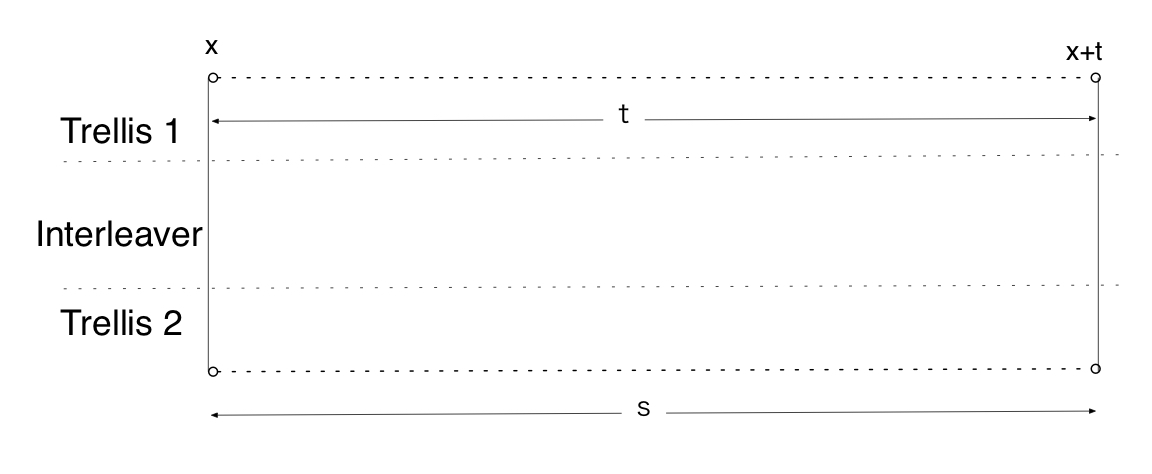
\includegraphics[width=8cm]{weight2.jpg}
\caption{$t=s=\tau$のエラーイベント}
\label{2_error}
\end{figure}
\end{center}

$s$ is calculated using the equation below.
\begin{equation}
\begin{split}
s&=\Pi_{\mathbf{L}_n}(x+t)-\Pi_{\mathbf{L}_n}(x)\\
&=b(x+t)-b(x) \mod N\\
&=bt \mod N
\label{three}
\end{split}
\end{equation}

The weight of the codeword can be calculated using the equation below.
\begin{equation}
d_{(t_i,s_j)}=w_o\Bigg( 3+\Bigg( \frac{ \left|t_i\right|}{\tau} + 
\frac{ \left|s_j\right|}{\tau} \Bigg)\Bigg)
\label{four}
\end{equation}

Substituting (\ref{three}) into (\ref{four}) and rewriting $t$ as $\tau$ gives
\begin{equation}
d_{(t_i,s_j)}=w_o\Bigg( 3+\Bigg( 1+ \frac{ b\tau \mod N}{\tau} \Bigg)\Bigg)
\label{five}
\end{equation}

It should be noted that values of b that are considered should satisfy the condition
\begin{equation}
( (b\tau \mod N )\mod \tau ) \neq 0
\label{six}
\end{equation}

The process for choosing the value of b that changes the input to the second 
component encoder into the form in (\ref{one}) is outlined below.

\paragraph{1.} For a given value of $b$ , $\ 1 \leq b \leq N/2$ which 
satisfies (\ref{six}) and all possible inputs of the 
form $(1+D^{t\tau})(D^u) ,0\leq u\leq N-\tau, t=1$, 
calculate corresponding s using (\ref{three})
\paragraph{2.} Calculate the Hamming distance for the codeword using
 equation (\ref{four}) and select min $d_{(t_i,s_j)}$
\paragraph{3.}After min $d_{(t_i,s_j)}$ is selected for all possible values of b,
 the value of b which corresponds to max(min $d_{(t_i,s_j)_v}$)

\paragraph{}
The tables below show the values for b selected for $t=\tau$ and $t=2\tau$ for 
various frame sizes.
\csvautolongtable[
      table head=\caption{$N=2^{m}$, 
      $m = \{10, 11, 12, 13, 14\} $, $t=\tau$}\label{tab:t1}\\\hline
               \csvlinetotablerow\\\hline
               \endfirsthead\hline
               \csvlinetotablerow\\\hline
               \endhead\hline
               \endfoot,
               respect all
               ]{t_tau_1.csv}
               
               \csvautolongtable[
      table head=\caption{$N=2^{m}$, 
      $m = \{10, 11, 12, 13, 14\} $, $t=2\tau$}\label{tab:t2}\\\hline
               \csvlinetotablerow\\\hline
               \endfirsthead\hline
               \csvlinetotablerow\\\hline
               \endhead\hline
               \endfoot,
               respect all
               ]{t_tau_2.csv}


    
\section{References}
\paragraph{1}  Oscar Y. Takeshita, Member, IEEE, and Daniel J. Costello ,
''New Deterministic Interleaver Designs for Turbo Codes'',IEEE Trans. Inform. Theory,
 vol. 46,pp. 1988-2006,Nov. 2000\\
  \paragraph{2} L. C. Perez, J. Seghers, D. J. Costello, Jr., 
  ''A distance spectrum interpretation of turbo codes'', IEEE Trans. Inform. Theory,
   vol. 42, pp. 1698-1709, Nov. 1996.\\
\paragraph{3} Jing Sun, Oscar Y. Takeshita ”Interleavers for Turbo Codes Using 
Permutation Polynomials over Integer Rings”, IEEE Trans. Inform. Theory, vol. 51,
pp. 101 - 119 Jan. 2005\\
\paragraph{4} John G. Proakis, Masoud Salehi. ''Digital Communications'', 
Fifth Edition,Chapter 8, McGraw-Hill\\.

\end{document}